\begin{frame}{Language Models Memorize Training Data}
  \begin{itemize}\footnotesize\itemsep0.3em
    \item[\textcolor{red}{$\blacktriangleright$}] \textbf{Extractable memorization:} a training string $s$ is extractable with $k$ tokens of context if the training data contains $[p \,\|\, s]$ for some length-$k$ prefix $p$ and greedy decoding from $p$ returns exactly $s$. Example: ``My phone number is'' ($k=4$) completes to the number that followed it in training.
    \item[\textcolor{red}{$\blacktriangleright$}] \textbf{Three log-linear trends} (GPT-Neo, 125M to 6B, trained on the Pile): extraction rises with (a) model size, about 19 percentage points per tenfold increase; (b) copies of a string in the data; (c) prompt length: 33\% of sampled sequences are extractable from the 6B model with 50 tokens of context, 65\% with 450.
    \item[\textcolor{red}{$\blacktriangleright$}] \textbf{A memorization effect:} GPT-2, never trained on the Pile, completes about 6\% of the same sequences against 40\% for GPT-Neo 1.3B. Lower bound: GPT-J (6B) memorizes at least 1\% of the Pile.
  \end{itemize}
  \vspace{0.1em}
  {\centering
  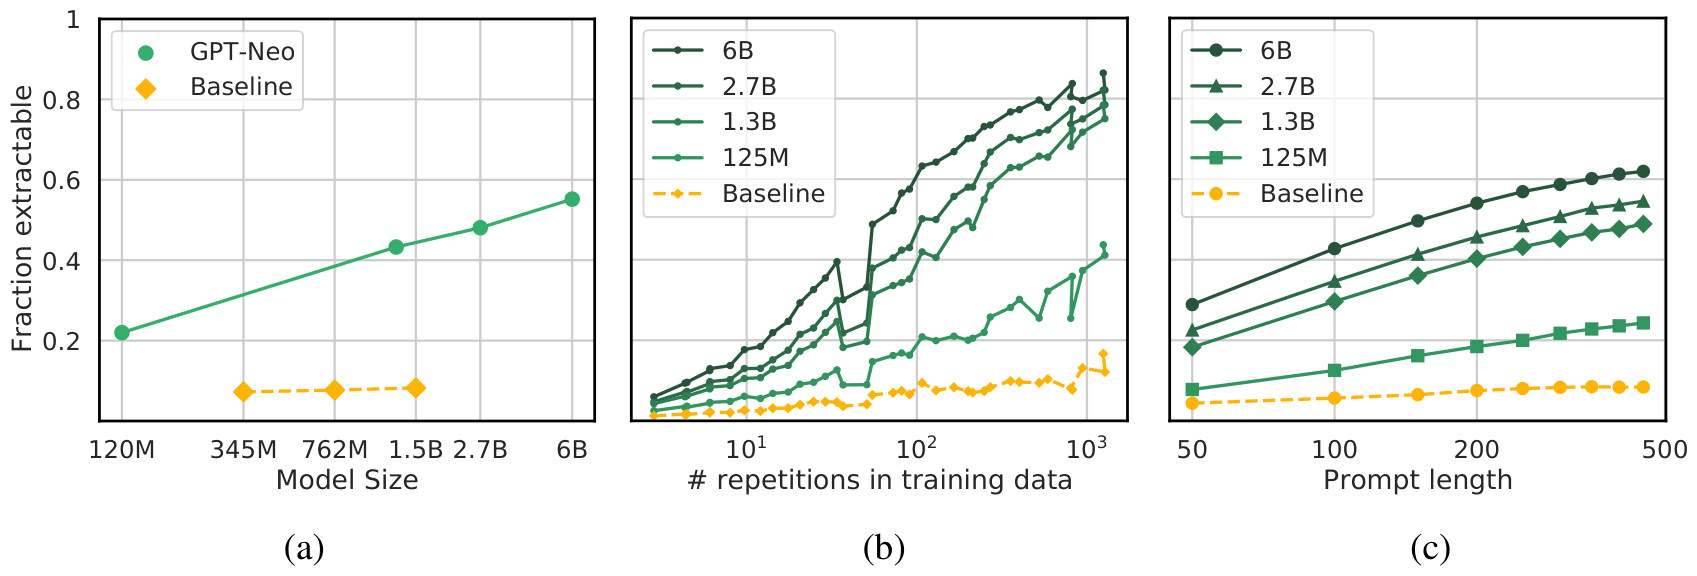
\includegraphics[width=\textwidth,height=0.34\textheight,keepaspectratio]{images/nlp-security-enterprise/quantifying_memorization_fig1_scaling.png}\\[0.1em]
  {\scriptsize Carlini et al., ``Quantifying Memorization Across Neural Language Models,'' ICLR 2023, \href{https://arxiv.org/abs/2202.07646v3}{arXiv:2202.07646v3}, Figure~1.\par}\par}
\end{frame}

\begin{frame}{Extracting Training Data: Generate, Rank, Verify}
  \begin{itemize}\footnotesize
    \item[\textcolor{red}{$\blacktriangleright$}] \textbf{Training-data extraction:} recovering individual training examples verbatim from query access alone. Carlini et al.\ attacked GPT-2, whose training data they could check with its creators.
  \end{itemize}
  \vspace{0.2em}
  {\centering
  \resizebox{\textwidth}{!}{%
  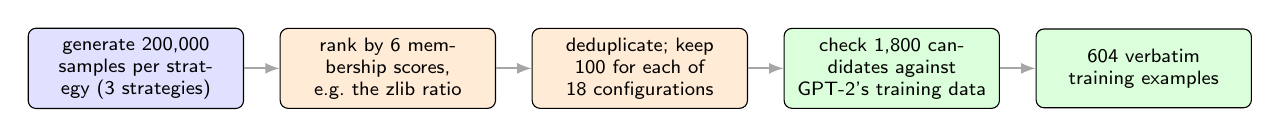
\begin{tikzpicture}[font=\sffamily\scriptsize, >=latex,
      stepnode/.style={draw, rounded corners=0.1cm, align=center, text width=2.5cm, minimum height=1.0cm},
      gennode/.style={stepnode, fill=blue!12},
      ranknode/.style={stepnode, fill=orange!16},
      checknode/.style={stepnode, fill=green!14},
      flowarr/.style={->, thick, gray!70}]
    \node[gennode]   (g) at (0,0)    {generate 200,000 samples per strategy (3 strategies)};
    \node[ranknode]  (r) at (3.2,0)  {rank by 6 membership scores, e.g.\ the zlib ratio};
    \node[ranknode]  (d) at (6.4,0)  {deduplicate; keep 100 for each of 18 configurations};
    \node[checknode] (v) at (9.6,0)  {check 1,800 candidates against GPT-2's training data};
    \node[checknode] (m) at (12.8,0) {604 verbatim training examples};
    \draw[flowarr] (g) -- (r);
    \draw[flowarr] (r) -- (d);
    \draw[flowarr] (d) -- (v);
    \draw[flowarr] (v) -- (m);
  \end{tikzpicture}}\par}
  \vspace{0.3em}
  \begin{columns}[T,onlytextwidth]
    \column{0.48\textwidth}
      \begin{itemize}\footnotesize
        \item[\textcolor{red}{$\blacktriangleright$}] \textbf{zlib score:} memorized text is easy for the model to predict yet hard to compress:
          \[ \mathrm{score}(x) = \frac{\log \mathrm{PPL}_{\text{GPT-2}}(x)}{\mathrm{zlib}(x)} \]
          $\mathrm{PPL}_{\text{GPT-2}}(x)$ is the perplexity of sample $x$ under GPT-2 and $\mathrm{zlib}(x)$ its size in bits after zlib compression. A low score means GPT-2 finds $x$ far more predictable than a generic compressor does.
      \end{itemize}
    \column{0.50\textwidth}
      \begin{itemize}\footnotesize\itemsep0.3em
        \item[\textcolor{red}{$\blacktriangleright$}] \textbf{Result:} 604 of the 1,800 candidates were verbatim training data (33.5\%; 67\% for the best configuration), some present in a single training document.
        \item[\textcolor{red}{$\blacktriangleright$}] \textbf{PII} (personally identifiable information: names, phone numbers, email and postal addresses, anything that identifies a person): 46 samples named individuals; 32 held contact details, 16 of them for private individuals.
      \end{itemize}
  \end{columns}
  \vspace{0.1em}
  {\scriptsize Carlini et al., ``Extracting Training Data from Large Language Models,'' USENIX Security 2021, \href{https://arxiv.org/abs/2012.07805v2}{arXiv:2012.07805v2}.}
\end{frame}

\begin{frame}{The Divergence Attack on ChatGPT}
  \begin{columns}[T,onlytextwidth]
    \column{0.52\textwidth}
      \begin{itemize}\footnotesize\itemsep0.35em
        \item[\textcolor{red}{$\blacktriangleright$}] \textbf{An aligned model looks private:} of 50 million tokens sampled from gpt-3.5-turbo, only 0.02\% were part of a 50-token sequence found in a 9\,TB corpus of public training data.
        \item[\textcolor{red}{$\blacktriangleright$}] \textbf{Divergence attack:} a prompt that pushes a chat model out of its dialogue behaviour and back to plain language modelling. Asked to repeat the word \texttt{poem} forever (the prompt lists it 50 times), the model repeats it several hundred times, then diverges, and part of what follows is copied from training data. Only single-token words work.
        \item[\textcolor{red}{$\blacktriangleright$}] \textbf{Result:} \$200 of queries recovered over 10,000 unique verbatim training examples, a rate 150 times higher than under normal use; 16.9\% of 15,000 labelled generations contained memorized PII. Alignment hid the memorized data without removing it.
      \end{itemize}
    \column{0.46\textwidth}
      \centering
      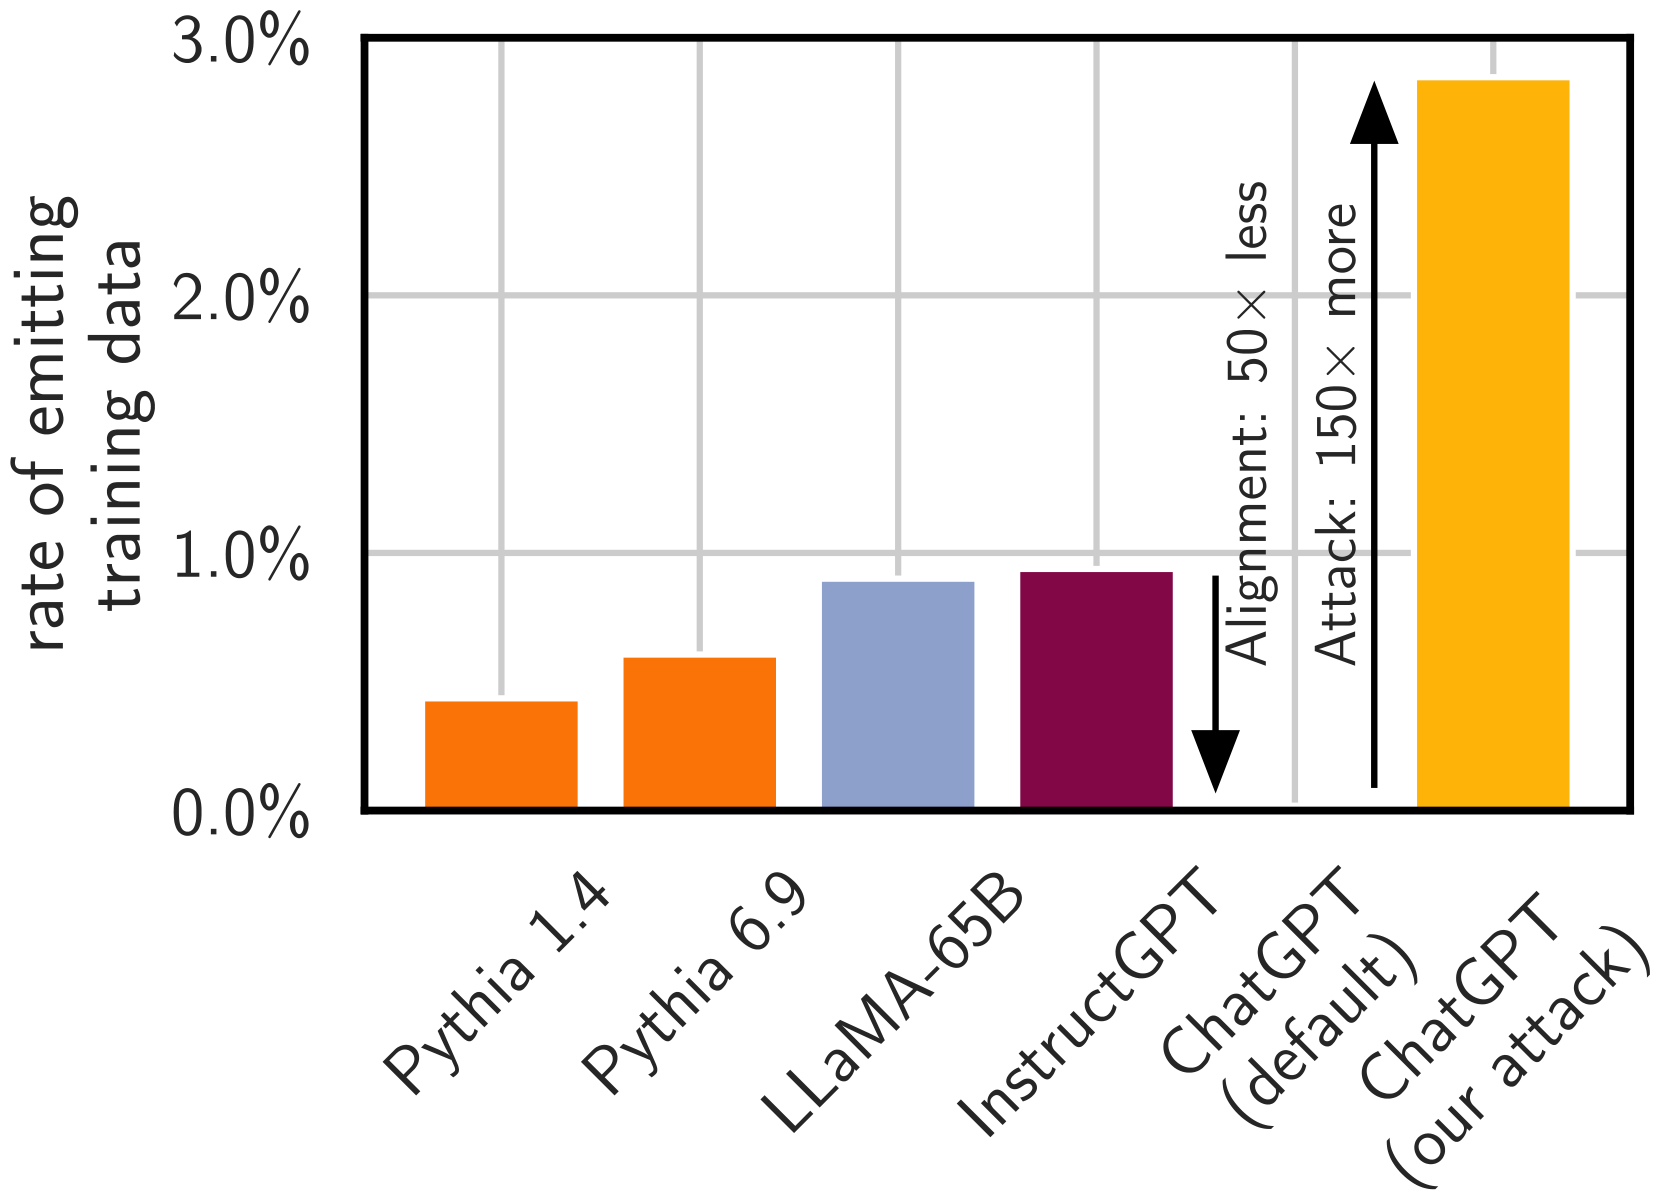
\includegraphics[width=\linewidth,height=0.56\textheight,keepaspectratio]{images/nlp-security-enterprise/scalable_extraction_fig1_emission_rate.png}\\[0.2em]
      {\scriptsize Rate of emitting training data by model, with ChatGPT before and after the attack. Nasr et al., ``Scalable Extraction of Training Data from (Production) Language Models,'' arXiv 2023, \href{https://arxiv.org/abs/2311.17035v1}{arXiv:2311.17035v1}, Figure~1.\par}
  \end{columns}
\end{frame}

\begin{frame}{Membership Inference and Its Limits}
  \begin{itemize}\footnotesize\itemsep0.2em
    \item[\textcolor{red}{$\blacktriangleright$}] \textbf{Membership inference attack (MIA):} given a record $x$ and query access to a model $M$, decide whether $x$ was in $M$'s training set by thresholding a score $f(x;M)$. Contamination tests ask the same question of a whole benchmark.
    \item[\textcolor{red}{$\blacktriangleright$}] \textbf{Loss attack} (Yeom et al.): predict ``member'' when the loss of $M$ on $x$ is low. If the loss is at most $B$ and the attack says ``non-member'' with probability equal to the loss divided by $B$, its membership advantage (true-positive minus false-positive rate) is the generalization gap over $B$: overfitting leaks membership.
    \item[\textcolor{red}{$\blacktriangleright$}] \textbf{Min-K\% Prob} (Shi et al.): unseen text tends to contain a few outlier tokens of very low probability, so score $x$ by its least likely tokens:
      \[ \text{Min-}K\%\,\text{Prob}(x) = \frac{1}{E} \sum_{x_i \in \text{Min-}K\%(x)} \log p(x_i \mid x_1, \ldots, x_{i-1}) \]
      $\text{Min-}K\%(x)$ is the set of the $k\%$ tokens of $x$ with the lowest probability, $E$ its size, and $p$ the model's next-token probability. A high score suggests membership; $k = 20$ worked best.
    \item[\textcolor{red}{$\blacktriangleright$}] \textbf{Caveat} (Duan et al.): against deduplicated Pythia models (160M to 12B) on Pile data, no MIA beat an AUC of 0.6 outside GitHub code (0.5 is chance): about one pass over a huge corpus leaves little per-record signal. Shi et al.'s high scores likely reflect non-members drawn from a later period.
  \end{itemize}
  \vspace{0.1em}
  {\scriptsize Yeom et al., CSF 2018, \href{https://arxiv.org/abs/1709.01604v5}{arXiv:1709.01604v5}; Shi et al., ICLR 2024, \href{https://arxiv.org/abs/2310.16789v3}{arXiv:2310.16789v3}; Duan et al., COLM 2024, \href{https://arxiv.org/abs/2402.07841v2}{arXiv:2402.07841v2}.}
\end{frame}

\begin{frame}{Differential Privacy and DP-SGD}
  \begin{columns}[T,onlytextwidth]
    \column{0.48\textwidth}
      \begin{itemize}\footnotesize\itemsep0.2em
        \item[\textcolor{red}{$\blacktriangleright$}] \textbf{Neighbouring datasets} $D, D'$: identical except for one record, present in one and absent from the other.
        \item[\textcolor{red}{$\blacktriangleright$}] \textbf{$(\varepsilon,\delta)$-differential privacy:} a randomized training algorithm $M$ satisfies it if, for all neighbours $D, D'$ and every set $S$ of outputs,
          \[ \Pr[M(D) \in S] \leq e^{\varepsilon} \Pr[M(D') \in S] + \delta . \]
          $\varepsilon$ bounds how far one record can shift the distribution of trained models (smaller is more private); $\delta$ is the chance that the bound fails, preferably below $1/N$ for $N$ records.
        \item[\textcolor{red}{$\blacktriangleright$}] \textbf{Cost:} 97\% against 98.3\% non-private on MNIST and 73\% against about 80\% on CIFAR-10, at $(\varepsilon,\delta) = (8, 10^{-5})$; per-example gradients also cost memory and time.
      \end{itemize}
    \column{0.50\textwidth}
      \begin{itemize}\footnotesize\itemsep0.2em
        \item[\textcolor{red}{$\blacktriangleright$}] \textbf{DP-SGD} (Abadi et al.): each step samples a random group, a \textbf{lot}, taking each example with probability $L/N$; it clips every per-example gradient, $\bar g_i = g_i / \max(1, \|g_i\|_2 / C)$, adds noise and steps:
          \[ \tilde g = \frac{1}{L}\Big(\sum_i \bar g_i + \mathcal{N}(0, \sigma^2 C^2 I)\Big), \quad \theta \leftarrow \theta - \eta\, \tilde g \]
          $\theta$: parameters; $L$: expected lot size; $C$: clipping norm; $\sigma$: noise multiplier; $I$: identity matrix; $\eta$: learning rate. The moments accountant accumulates the privacy cost of every step into the final $(\varepsilon,\delta)$.
        \item[\textcolor{red}{$\blacktriangleright$}] \textbf{Language models:} Li et al.\ fine-tune GPT-2 and RoBERTa at $\varepsilon \in \{3, 8\}$; with large batches some DP models beat strong non-private baselines; ghost clipping (per-example gradient norms without storing per-example gradients) keeps memory near non-private levels.
      \end{itemize}
  \end{columns}
  \vspace{0.1em}
  {\scriptsize Abadi et al., ``Deep Learning with Differential Privacy,'' CCS 2016, \href{https://arxiv.org/abs/1607.00133v2}{arXiv:1607.00133v2}; Li et al., ICLR 2022, \href{https://arxiv.org/abs/2110.05679v6}{arXiv:2110.05679v6}.}
\end{frame}

\begin{frame}{Privacy Controls in a Deployed LLM}
  \centering
  {\scriptsize
  \begin{tabular}{>{\raggedright\arraybackslash}p{1.5cm} >{\raggedright\arraybackslash}p{4.2cm} >{\raggedright\arraybackslash}p{6.4cm}}
    \toprule
    \textbf{Stage} & \textbf{Control} & \textbf{Evidence and limit} \\
    \midrule
    Training data & Deduplicate sequences & Deduplicated models emit 20$\times$ less training data; a sequence seen 10 times is generated about 1000$\times$ more often than one seen once (Kandpal et al.) \\
    \addlinespace[0.2em]
    Training data & Scrub PII with entity taggers, replacing each hit with a mask token & Reduces but does not prevent leakage; sentence-level DP still leaked about 3\% of PII sequences, since PII repeats across records (Lukas et al.) \\
    \addlinespace[0.2em]
    Training & Train with DP-SGD & VaultGemma 1B ($\varepsilon \leq 2.0$, $\delta \leq 1.1 \times 10^{-10}$ per 1024-token sequence): no memorization detected; ARC-E 51.8, close to GPT-2 1.5B (51.1) and below non-private Gemma 3 1B (71.3) \\
    \addlinespace[0.2em]
    Deletion & Machine unlearning: fine-tune the model to forget a set of examples, without retraining & TOFU (200 fictitious authors): no baseline matched a model never trained on the forget set ($p < 0.01$ even for a 1\% forget set) \\
    \addlinespace[0.2em]
    Inference & Redact PII before external APIs; filter outputs for PII; retention rules for prompt logs & Keeping prompts in-house: on-premises deployment \\
    \bottomrule
  \end{tabular}\par}
  \vspace{0.3em}
  {\scriptsize Kandpal et al., ICML 2022, \href{https://arxiv.org/abs/2202.06539v3}{arXiv:2202.06539v3}; Lukas et al., IEEE S\&P 2023, \href{https://arxiv.org/abs/2302.00539v4}{arXiv:2302.00539v4}; VaultGemma Team, \href{https://arxiv.org/abs/2510.15001v2}{arXiv:2510.15001v2}, Table~2; Maini et al., \href{https://arxiv.org/abs/2401.06121v1}{arXiv:2401.06121v1}.}
\end{frame}
